\chapter{Simultaneous Localization and Mapping}
\label{chapter:slam}

\textbf{Author: Lukas Leskovar} 

%frame of reference klingt nicht so gut
The problem of localizing as well as navigating a system through a completely or partly unknown environment without any external coordinate system (i.e. GPS, Optical Beacon Tracking, etc.) has proven itself to be one of the most complex and yet fundamental topics in many scientific research fields with robotics being most prominent. The main approach to this problem is Simultaneous Localization and Mapping (SLAM) which dates back to the mid 1980s. Back then the first solutions based on Extended Kalman Filters or Rao-Blackwellised Filters were formulated. \footcite{durrantSlam2006}  \footcite{cadenaSlamFuture2016}

To date the topic of SLAM has matured, algorithms have gotten more reliable and robust and are utilized in many industries. Applications for SLAM range from navigating a Mars-Rover over autonomous cars or warehouse robots to simple household appliances like vacuum cleaners. 

As one major topic of this thesis is robot navigation in a GPS-denied area as well as mapping of such environment, different modern SLAM approaches and solutions utilized by the project team are discussed in this chapter.

\section{Localization}
%state estimation beschreiben dass pose sowie andere informationen wie geschw. usw. erfasst werden. 
Localization or state-estimation aims to reconstruct the state of a system using interoceptive measurements (e.g. acceleration, velocity, etc.) as well as an exteroceptive model (e.g. position and orientation) of the system. \footcite{barfootStateEstimation2017}
Put into the context of mobile robotics this means that in order to perform comprehensive localization of a mobile robot a sensor fusion between on-board sensors and a global coordinate system ought to be performed as solely relying on sensor data such as odometry would quickly result in large accumulated errors.
%Exemplary for such a robot would be a drone utilizing a Inertial Measurement Units (IMU) odometry as well as GPS positional data to estimate its current position.
An exemplary system for this would be an industrial robot utilizing a construction plan to correct errors by wheel-encoded odometry to navigate through a factory. 

\section{Mapping}
Contrary to localization, in mapping problems the current pose of the system is known while its environment remains uncharted.
Therefore stand-alone mapping aims to generate a model of its environment by evaluating sensor readings of environmental features as well as the systems pose to reconstruct aforementioned features in a global reference frame. 
Mapping applications often combine technologies typically found in other scientific fields such as photogrammetry or computer vision.
An example for such a system would be a drone computing camera images and GPS positional data with a photogrammetric algorithm to reconstruct a 3D-Model of a building. 


\section{Localization and Mapping}
The aforementioned technologies on their own are considered rather simplistic problems as either the environments map is given or a reliable pose-estimation can be provided. While most applications meet either of these criteria with pre-built maps or GPS being available, some environments such as buildings, mineshafts or outer space both the systems pose and environment remain uncertain and need to be determined simultaneously hence the name Simultaneous Localization and Mapping. 
To summarize, the crux of the SLAM problem, as described in Fig. \ref{fig:slamOverview}, is that localizations requires a map and mapping depends on pose estimates however neither are certain. 

%The following sections will mainly focus on the SLAM back-end and dissect the problem by reviewing different probabilistic approaches. 


%In order to partially solve this dilemma SLAM incorporates loop closure to correct the global map as well as positional estimates provided by odometry. A loop closure event occurs when revisiting previously mapped landmarks and associating relations between features to adapt the global topology. %Without loop closure a mobile robot would perceive its environment as a infinite corridor.


\begin{figure}
	\centering
	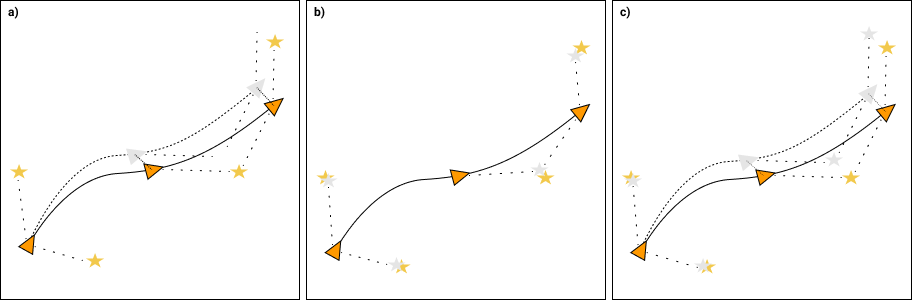
\includegraphics[width=1.0\linewidth]{img/slamOverview}
	\caption{
		The figure above depicts the different tasks contributing to the SLAM problem. Panel a) shows a robot (triangles) moving trough a known environment while the pose and path remain uncertain. In panel b) the robots pose is certain while the landmark (stars) locations need to be determined. Panel c) composes both previous problems where neither the robot state nor the landmark locations are certain. \footcite{durrantSlam2006}
	}
	\label{fig:slamOverview}
\end{figure}

\section{Map Representation}
The way a robot perceives its surroundings and maintains a accurate map is directly dependant on many criteria such as complexity of tasks, size of its environment as well as measurement quality mainly influenced by sensor noise. 
Tailoring to benefit some of the aforementioned criteria most robotic mapping systems utilize either of two paradigms, metric or topological, each proposing their respective strengths and weaknesses.

Metric or grid-based maps build a map of the robots environment as occupancy grids, with each cell indicating the presence of an obstacle. The main benefit using metric maps is the facilitated construction of large-scale mappings as well as non-ambiguous determination of places. However such maps have significant drawbacks concerning space as well as time complexity and require accurate pose estimation of the robot.

Topological or feature-based maps reconstruct their environment as graphs with each node representing a feature or landmark perceived by the robots sensors. In contrast to metric maps they allow for comprehensive path planning and are significantly more compact as its resolution is directly proportional to the environments complexity. \footcite{thrunMaps1998}


\section{Probabilistic Definition}
To describe probabilistic SLAM lets assume a robot is moving through an environment observing multiple landmarks at different times. 
The goal is that, for any time instant $ t $, the robots state vector 
\[ x_{t} = 
\begin{pmatrix}
	x \\
	y \\
	\theta \\
\end{pmatrix}
\] as well as a time invariant set of all absolute landmark positions 
% describing its position and orientation as well as a time invariant set of all absolute landmark positions 
% umformulieren dass es nicht heißt der state vector beschreibt die landmarks
$ m = \{ m_{1}, m_{2}, ..., m_{i} \}$ 
is computed, given uncertain relative landmark observations $ z_{0:t} = \{z_{0}, z_{1}, ..., z_{t}\}$, controls $ u_{0:t} = \{u_{0}, u_{1}, ..., u_{t}\}$ and known initial location $ x_{0} $. Fig. \ref{fig:slamGraphical} depicts this process and illustrates the relationships between the variables important in any SLAM system. 

\begin{equation}\label{fullSLAM}
	P(x_{0:t}, m | z_{0:t}, u_{0:t}, x_{0})
\end{equation}

In \ref{fullSLAM}, which is often referred to as "Full-SLAM" or "Offline-SLAM", the joint posterior density of the robots trajectory and landmark locations is estimated. In other words, this formulation of the problem aims to recover the whole robot trajectory.

\begin{equation}\label{onlineSLAM}
	P(x_{t}, m | z_{0:t}, u_{0:t}, x_{0})
\end{equation}

The pendant to this is "Online-SLAM" which aims estimate only the robots latest location at time instant $ t $, as seen in \ref{onlineSLAM}. In contrast to "Full-SLAM", performing batch computation on the whole data, algorithms pursuing this online approach typically compute the probability distribution incrementally. 

\begin{figure}
	\centering
	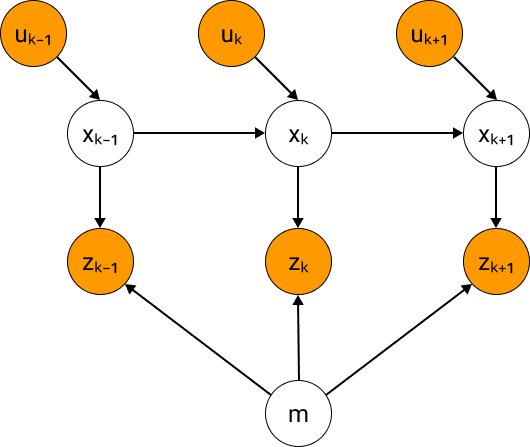
\includegraphics[width=0.4\linewidth]{img/SlamGraphical}
	\caption{
		A Bayes network graph depicting the causal relationships between sensor measurements (orange circles) and uncertain variables (white circles). It is made apparent how the relative measurements by odometry or landmark observation influence the robot state as well as landmark locations. 
	}
	\label{fig:slamGraphical}
\end{figure}

To compute either problem a mathematical model representing the robots state transition and a model describing observations ought to be defined:

\begin{equation}\label{motionModel}
	P(x_{t} | x_{t-1}, u_{t})
\end{equation}

\begin{equation}\label{observationModel}
	P(z_{t} | x_{t}, m)
\end{equation}

The motion model \ref{motionModel} describes the robots location at time $ t $ given a known previous location $ x_{t-1} $ and control $ u_{t} $ assuming the state-transition is a Markov process \footcite{haeneltMarvoModel2006}.
\ref{observationModel} calculates the probability of observing a landmark $ z_{t} $ when the robots location $ x_{t} $ and environment $ m $ are known.
\footcite{durrantSlam2006}
 %For aforementioned reasons in SLAM the map is not known to the system, therefore many formulations omit the map in the observation model.

%The joint posterior is then implemented in a recursive prediction and correction form which is often described as time-update and measurement-update:

For filtering approaches which are discussed later in this chapter, the joint posterior is then implemented in a recursive prediction and correction form which is often described as time-update and measurement-update:

\begin{equation}\label{timeUpdate}
	P(x_{t}, m | z_{0:t-1}, u_{0:t}, x_{0}) = \int P(x_{t} | x_{t-1}, u_{t}) P(x_{t-1}, m | z_{0:t-1}, u_{0:t-1}, x_{0}) dx_{t-1}
\end{equation}


\begin{equation}\label{measurementUpdate}
	P(x_{t}, m | z_{0:t}, u_{0:t}, x_{0}) = \frac{P(z_{t} | x_{t}, m) P(x_{t}, m | z_{0:t-1}, u_{0:t}, x_{0}))}{P(z_{t} | z_{0:t-1}, u_{0:t}}
\end{equation}

The time update in \ref{timeUpdate} calculates an estimate of the robots state using a previously known state at $ t - 1 $ and state-transition given the newest control $ u_{t} $.
In the next step, the measurement update \ref{measurementUpdate}, a observation $z_{t} $ is taken and the previously calculated estimate is corrected using Bayes-Theorem\footcite{durrantSlam2006}. 

To make the the recursive structure of such filtering approaches more apparent the equations \ref{timeUpdate} and \ref{measurementUpdate} can be compared to the Bayes filter algorithm, commonly used as framework for further state-estimation problems\footcite[Page 23]{thrun2002probabilisticRobotics}.

\begin{equation}\label{timeUpdateBayes}
	\overline{\rm bel}(x_{t}) = \int P(x_{t} | x_{t-1}, u_{t})  bel(x_{t-1}) dx_{t-1}
\end{equation}


\begin{equation}\label{measurementUpdateBayes}
	bel(x_{t}) = \eta  P(z_{t} | x_{t})  \overline{\rm bel}(x_{t-1})
\end{equation}

\section{Solution Paradigms} 
Over time many different approaches to the SLAM problem have been developed which can be categorized into either of three paradigms. The two mature ones are based on recursive filtering techniques while the modern graph-based solutions perform non-linear sparse optimization.

\subsection{Extended Kalman Filter}
\label{sec:ExtendedKalmanFilter}
The Extended Kalman Filter (EKF) is one of the first approaches to the Online-SLAM problem and a extension of the Kalman Filter (KF). Contrary to the standard KF it is applicable to non-linear systems by performing linear approximation.

%The Extended Kalman Filter (EKF) is one implementation of a Bayes Filter for non-linear problems and was one of the first approaches to the Online-SLAM problem. The author recommends preliminary knowledge about Bayes Filters\footcite{tipaldiBayes2020}, the vanilla Kalman Filter and the EKF\footcite{tipaldiEKF2020} before reading this section about its application in SLAM. 

The Kalman Filter assumes a environment in which landmarks can be fully represented as points within the coordinate frame. The earlier introduced state-vector $ x $ is extended to a state-space vector with dimensions $ 3 + 2n$
\[ \mu = 
\begin{pmatrix}
	x \\
	m \\
\end{pmatrix}
=
\begin{pmatrix}
	x & y & \theta & m_{1, x} & m_{1, y} & \dots & m_{n, x} & m_{n, y} 
\end{pmatrix} ^{T}
\] 
to incorporate $n$ landmark locations. 

Furthermore a covariance matrix 
$ \Sigma = 
\begin{pmatrix}
	\Sigma_{xx} & \Sigma_{xm} \\
	\Sigma_{mx} & \Sigma_{mm} \\
\end{pmatrix} $ 
is introduced which specifies the state $ x $ and landmark $ m $ uncertainties as well as correlations between landmarks and robot pose. 

The motion and observation models are implemented as non-linear functions $x_{t} = g(u_{t}, x_{t - 1}) + \epsilon_{t}$ and $z_{t} = h(x_{t}) + \delta_{t}$ with $\epsilon_{t}$ and $\delta_{t}$ defined as random noise variables.% commonly based on zero-mean additive Gaussian noise.

%defined as non-linear Gaussian distributions $ \mathcal{N}(g(u_{t}, x_{t - 1}), R_{t}) $ and $ \mathcal{N}(h(x_{t}), Q_{t}) $ based on non-linear functions $g$ and $h$ with $ R_{t} $ and $ Q_{t} $ representing zero-mean additive Gaussian noise.
To still calculate the state transition as well as measurement update these functions are linearized by performing first order Taylor Expansion\footcite[Pages 33-51]{thrun2002probabilisticRobotics}.

%\begin{equation}
%	g(u_{t}, x_{t - 1}) \approx g(u_{t}, \mu_{t - 1}) + g'(u_{t}, \mu_{t - 1})(x_{t - 1} - \mu_{t - 1}) 
%	= g(u_{t}, \mu_{t - 1}) + G_{t}(x_{t - 1} - \mu_{t - 1})
%\end{equation}
%
%\begin{equation}
%	h(x_{t}) \approx h(\overline{\mu}_{t}) + h'(\overline{\mu}_{t})(x_{t} - \overline{\mu}_{t}) 
%	= h(\overline{\mu}_{t}) + H_{t}(x_{t} - \overline{\mu}_{t})
%\end{equation}

This allows for the functions to be incorporated in the vanilla Kalman Filter Algorithm which consists of the following five step procedure:

\begin{algorithm}[H]
	\caption{Pseudo-Code describing the filter cycle of a Extenden Kalman Filter\footcite[Page 51]{thrun2002probabilisticRobotics}}
	\SetKwFunction{FMain}{ExtendedKalmanFilter}
	\SetKwProg{Fn}{Function}{:}{}
	
	\Fn{ \FMain{ $\mu_{t - 1}$, $\Sigma_{t-1}$, $u_{t}$, $z_{t}$ } } 
	{
		$ \overline{\mu}_{t} \gets g( u_{t}, \mu_{t - 1} ) $\;
		$ \overline{\Sigma}_{t} \gets G_{t} \Sigma_{t-1} G^{T}_{t-1} + R{t} $\;
	
		$ K_{t} \gets \overline{\Sigma}_{t} H^{T}_{t} ( H_{t} \overline{\Sigma}_{t} H^{T}_{t} + Q_{t} )^{-1} $\;
		$ \mu_{t} \gets \overline{\mu}_{t} + K_{t} ( z_{t} - h( \overline{\mu}_{t} ) ) $\;
		$ \overline{\Sigma}_{t} \gets ( I - K_{t} H_{t} ) \overline{\Sigma}_{t} $\;
		
		\Return $\mu_{t}$, $\Sigma_{t}$\;
	}
	\textbf{End Function}	
\end{algorithm}

Notice that the Jacobian matrices $G_{t}$ and $H_{t}$ containing all partial derivatives of $g$ and $h$ are utilized describing the transformation of robot state as well as observations based on the pose.

%\begin{itemize}
%	\item State Prediction: The next state $ \mu_{k} $ is predicted given the controls $ u_{k} $ and previous state $ \mu_{k-1} $.
%	\item Measurement Prediction: A prediction of the next measurement is made propagating the uncertainty introduced by the state-transition.
%	\item Measurement: A new measurement is taken.
%	\item Data Association: The error between the prediction and actual measurement is calculated.
%	\item Update: The state-space vector as well as covariance matrix is updated given the previously calculated error. This update then reduces the uncertainty of both robot state and landmark locations.
%\end{itemize} 


%wenn noch platz bleibt darüber schreiben dass taylor expansion nicht so gut ist

\subsection{Particle Filter}
One major problem with the EKF paradigm is its inability to perform estimations under non-Gaussian distributions. 
To this end particle filters estimate a specific probability distribution by proposing multiple hypothesis which get continuously more accurate as the algorithm proceeds. 
Particle filtering for SLAM with algorithms like Fast-SLAM, is based on Monte-Carlo Localization (MCL) which is roughly described in the following steps:
\begin{itemize}
	\item For each state $ x_{t} $ a set 
	$
	\mathcal{X} = 
	\{ 
	\langle
	\begin{matrix}
		 x_{t}^{[j]},  \omega^{[j]}
	\end{matrix}
	\rangle
	, ...
	\}
	_{j=1, ..., J}
	$
	of particles or samples 
	with random state hypothesis is generated from a proposal distribution. %welche?
	\item The probability for each particle to be representing the true state is calculated by comparing its estimation with a measurement thus yielding in each particles importance weight $ \omega^{[j]} $.
	\item The last step is to remove samples with a lower likelihood and add more samples in regions with higher importance weights, this process is called resampling and shares many similarities with survival of the fittest algorithms.
\end{itemize}

%nur kleiner satz der mir eingefallen ist
Because the number of particles greatly affects the performance of a particle filter, such approaches perform best in low dimension spaces. To this end the Fast-SLAM algorithm utilizes Rao-Blackwellization, see Equation \ref{RaoBlackwellization}, to separate the joint probability of robot state and map into individual distributions which can be computed with much more ease.
This means that given the robots poses all landmarks are independent, which is described in Fig. \ref{fig:fastSlamGraphical}.

\begin{equation}\label{RaoBlackwellization}
	P(x_{0:t}, m | z_{0:t}, u_{0:t}) = P(x_{0:t} | z_{0:t}, u_{0:t}) P(m | x_{0:t}, z_{0:t})
\end{equation}

Following this approach the robots path is estimated by performing a Monte-Carlo localization drawing samples from the robots motion model $x_{t}^{[j]} \sim P(x_{t} | x_{t-1}^{[j]}, u_{t}) $. Besides the state information each particle maintains a set of landmarks, each represented as a low dimensional EKF. Therefore the importance weight for each particle corresponds to the accuracy between expected measurement and landmark observation as $ \omega^{[j]} \sim P(z_{t} | x_{t}^{[j]}, \overline{z}_{t}) $.
% therefore the importance weight for each particle corresponds to the joint accuracy of all landmark estimations. 
The final algorithm functions exactly as described with the exception that it incorporates the aforementioned EKF to estimate the landmark locations and compute the particle weight before updating its belief on landmark locations and initiating the resampling process \footcite[Pages 1159-1162]{stachniss2016simultaneous}. 


\begin{figure}
	\centering
	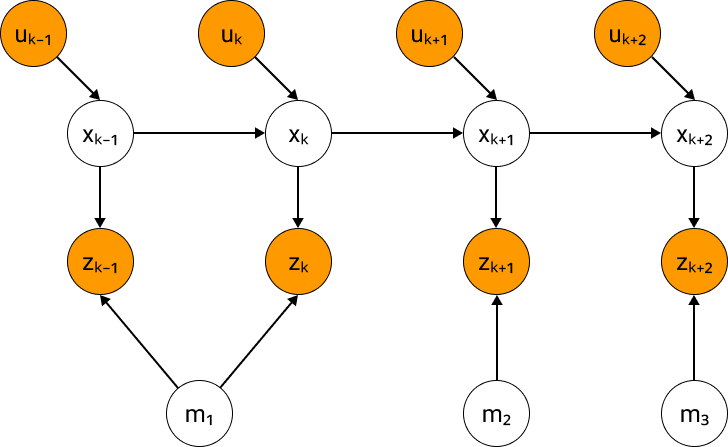
\includegraphics[width=0.5\linewidth]{img/FastSlamGraphical}
	\caption{
		This graphical description of the SLAM problem shows the assumption that the landmark estimates are all mediated through the robot path thus allowing for easier implementation by using smaller Gaussians for each landmark $m_{i}$ rather than a larger state-space vector as in EKF SLAM.
	}
	\label{fig:fastSlamGraphical}
\end{figure}

\subsection{Graph-based}
The newest paradigm to solve the offline SLAM problem are graph-based methods that essentially use a non-linear least-squares approach to compute the graph of poses best fitting the measurements. 
To this end the SLAM posterior is described as a graph of robot poses $ x_{i} $ at time $ t_{i} $ as nodes connected by soft constraints that correspond to spatial measurements $z_{ij}$ between two states.
These edges are generated in the following two cases:

\begin{equation}\label{odometryEdge}
	(X_{i}^{-1}X_{i+1})
\end{equation}

\begin{equation}\label{observationEdge}
	(X_{i}^{-1}X_{j})
\end{equation}

Here \ref{odometryEdge} corresponds to a edge based on odometry transformations by moving the robot from state $X_{i}$ to $X_{i+1}$, both of which are represented as vectors relative to the coordinate origin.
These transformations are illustrated in more detail in Fig. \ref{fig:poseGraphTransformation}.
The more interesting case is when an observation of a previously captured area occurs and a virtual measurement \ref{observationEdge} is computed, describing how the states $X_{j}$ and $X_{i}$ relate to each other according to the displacement between their observations, see Fig. \ref{fig:poseGraphOptimization}.

\begin{figure}
	\centering
	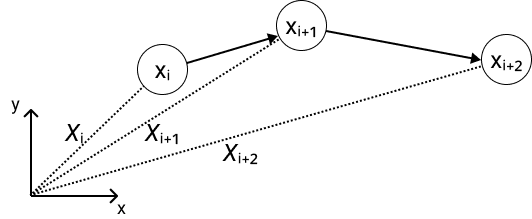
\includegraphics[width=0.6\linewidth]{img/PoseGraphTransformation}
	\caption{
		The graph of robot poses connected to each other by odometry measurements. To calculate the relative movement between two nodes each node can be represented as a matrix $X_{i}$ describing how it is transformed relative to the global coordinate frame.
	}
	\label{fig:poseGraphTransformation}
\end{figure}



This approach marginalizes any data about the map other than the correspondence of poses to primarily focus on solving the robot path. 
Given the pose-graph the goal is to compute the node configuration that minimizes the error between predicted edges, see \ref{observationEdge}, and actual measurements 
$
\langle
\begin{matrix}
	z_{ij},  \Omega_{ij}
\end{matrix}
\rangle
$, with the information matrix $\Omega_{ij}$ describing the measurement noise.

Equation \ref{leastSquares} describes this optimization process, with the error function $e_{ij}$ defined as any non-linear function essentially calculating the difference between estimate and true measurement for any pair of nodes. 
Once the optimal pose-graph is constructed the map data is rendered given known poses thus reducing the problem to simple mapping\footcite{grisetti2010graphSLAM}.

\begin{equation}\label{leastSquares}
	x* = argmin_{x} \sum_{ij}e_{ij}^{T} \Omega_{ij} e_{ij}
\end{equation}


\begin{figure}
	\centering
	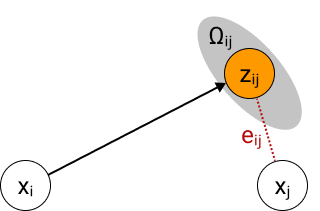
\includegraphics[width=0.4\linewidth]{img/PoseGraphOptimization}
	\caption{
		This pose-graph with two nodes describes how any pair of nodes are related to each other given a measurement. The measurement $ z_{ij} $ corresponds to how the node $x_{j}$ should be placed relative to node $x_{i}$ given that each of them share a similar observation. As seen in the figure this is not the case, thus demanding for the error $e_{ij}$ to be minimized. In other words, by moving the node $x_{j}$ closer to the optimum minimizes the error and corrects the pose-graph. \footcite{grisetti2010graphSLAM}
	}
	\label{fig:poseGraphOptimization}
\end{figure}


\section{Graph-SLAM topology}
%!!!!!! Front-End Backend Trennung ist nur bei graph based der Fall
Most modern graph-based SLAM systems are partitioned into the following modules:
\begin{itemize}
	\item A front-end in charge of abstracting sensory input by performing feature extraction as well as data association, further described in Section \ref{dataAssociation}. Essentially it constructs the pose-graph and feeds it into the back-end.
	%Furthermore it is responsible for associating corresponding features over multiple measurements, which is typically referred to as short-term data association. Long-term data association or loop closure therefore aims to link current measurements to previously observed features thus  correcting accumulated odometry errors as well as adapting the global topology. 
	\item A back-end performing pose-graph optimization based on the abstracted data fed in by the front-end. The back-end also provides positional information about nodes to the front-end thus supporting loop closure detection. 
\end{itemize}

While the front-end remains application specific as the data abstraction depends on the sensors utilized by the robot, the same back-end can be applied for many different scenarios as the pose-graph optimization essentially represents a squared-error minimization and many elaborated algorithms such as Gauss-Newton can be utilized.

%and is implemented by least-square solving algorithms such as gradient decent 

%auch in section graph based schieben
\section{Data Association}\label{dataAssociation}
%While many aspects of the front-end remain application specific each SLAM system typically contains modules for data association in the two ways.
One key trait that all SLAM paradigms posses is to recognise similarities in measurements and correct the incremental odometry error after revisiting previously mapped areas. This process is referred to as loop-closing or long-term data-association and reduces the uncertainty of pose and map estimates thus qualifying it as a integral part of any SLAM problem. 

While loop-closures aim to detect large correspondences in the global map, short-term data-association is responsible for associating corresponding features over multiple measurements which helps establishing the pose-graph. 

\section{Hierarchical Pose-Graphs}
While building the pose-graph can be computed with relatively low effort, performing loop-closures is a computational heavy process. Which makes graph-based online SLAM solutions difficult to implement as robot state and map need to be estimated in real-time scenarios. To facilitate the data association process, the global map is partitioned into sub-maps thus allowing data-associations to be calculated only in parts of the graph the robot is currently present. 

\section{Comparison of SLAM Paradigms}
%The previous sections explained the basic structure of the three main approaches to the SLAM problem with the Extended Kalman Filter being the most mature. 

%In its basic implementation the algorithmic complexity of EKF-SLAM is tightly coupled to the size of the covariance matrix which grows quadratically as more landmarks are observed. Furthermore local linearization as utilized in this approach has many disadvantages as results can be very inconsistent. To solve this efficiency problem many optimization approaches have been implemented in the past years\footcite{bailey2006simultaneous}.

%Particle filtering methods such as Fast-SLAM solve many issues found in the EKF as they directly incorporate a non-linear process model instead of performing linearization beforehand. Although the number of particles needed may increase dramatically Fast-SLAM still performs well with linear  time-complexity which may even be improved by implementing a balanced binary tree to organize particles as Montemerlo\footcite{montemerlo2002fastslam} suggests. 

%Contrary the relatively modern graph-based approach inherently aims to solve the Full-SLAM problem as it performs pose-graph optimization on the whole graph. The main benefit of this solution is the decoupling of front- and back-end which allows it to be used in many different scenarios. 
%Although its basic implementation performs offline many newer approaches adjust the pose-graph in real-time which makes such solutions relatively similar to EKF-SLAM. 


The Extended Kalman Filter is a mature approach to the SLAM problem and has been implemented many times in different types of applications. However it does not only lack computational efficiency in its original implementation, see. Tab. \ref{tab:slamComparison}, but also has shown to be very problematic concerning consistent solution and robust data-association. 
These problems stem from the algorithm definition itself, firstly as local-linearization of non-linear problem impairs the system to reach complete convergence, e.g. all landmark uncertainties converging to zero. Secondly the data-association model of EKF assumes all landmarks to be fully identifiable from any point of view, which cannot be guaranteed in most real-life scenarios and renders data-association very fragile.
Fortunately the EKF has been improved and optimized to address some of the aforementioned issues\footcite{bailey2006simultaneous}.

Another paradigm proposed was Particle Filtering which essentially applies a survival of the fittest model to robot poses. Solutions like Fast-SLAM optimize MCL algorithm by decoupling landmarks and estimating them through individual EKFs. 
The main benefit of this solution is the utilization of a non-linear model and ability to perform even with non-Gaussian distributions. 
Although its computationally more efficient compared to the previous approach, one problem is the need for large amounts of particles to achieve high accuracy. Montemerlo suggest implementing a balanced binary tree to store and organize particles which improves the complexity of the algorithm to $O(J  \log  M)$ with $J$ representing the amount of particles and $M$ being the number of landmarks\footcite{montemerlo2002fastslam}.

Lastly mentioned was the graph-based approach to SLAM which has grown significant popularity due to its versatility and reusability in different applications. The robot posterior is modelled as a sparse pose-graph which is optimized using a least-squares algorithm and is solved offline after the whole robot path has been captured. Some newer algorithms try to manipulate the pose-graph in real-time to establish a graph-based online SLAM solution\footcite{stachniss2016simultaneous}.


\begin{table}[]
	\centering
	\begin{tabular}{|l|l|l|}
		\hline
		\textbf{Approach}   & \textbf{Problem}    & \textbf{Time Complexity} \\ \hline
		\textbf{EKF}        & online SLAM         & $O(M^{2})$               \\ \hline
		\textbf{Fast-SLAM}  & full \& online SLAM & $O(J M)$                 \\ \hline
		\textbf{Graph SLAM} & full  SLAM          & $O(|V| + |N|)$           \\ \hline
	\end{tabular}
	\caption{The three main SLAM solution paradigms in basic implementation compared by their computational complexity. Note that the quadratic time complexity of the EKF approach is caused by quadratically extending the covariance matrix as landmarks $M$ are added and updated throughout mapping \footcite{durrantSlam2006}.
	For Fast-SLAM the complexity concerning just the particles $J$ stays linear, however during every resampling step each particle including all landmark estimate $M$ contained within need to be copied\footcite{montemerlo2002fastslam}.
	Lastly the back-end for most graph SLAM solution is based on least-squares error minimization of the pose graph with $|N|$ nodes as robot poses and $|V|$ vertices as measurements between nodes thus rendering the computational complexity to be  $O(|V| + |N|)$ without utilized hierarchical pose-graphs as studied by Korovko and Robustov\footcite{korovko2021partial}. 
}
	\label{tab:slamComparison}
\end{table}

\section{SLAM in Autumn}

\begin{figure}
	\centering
	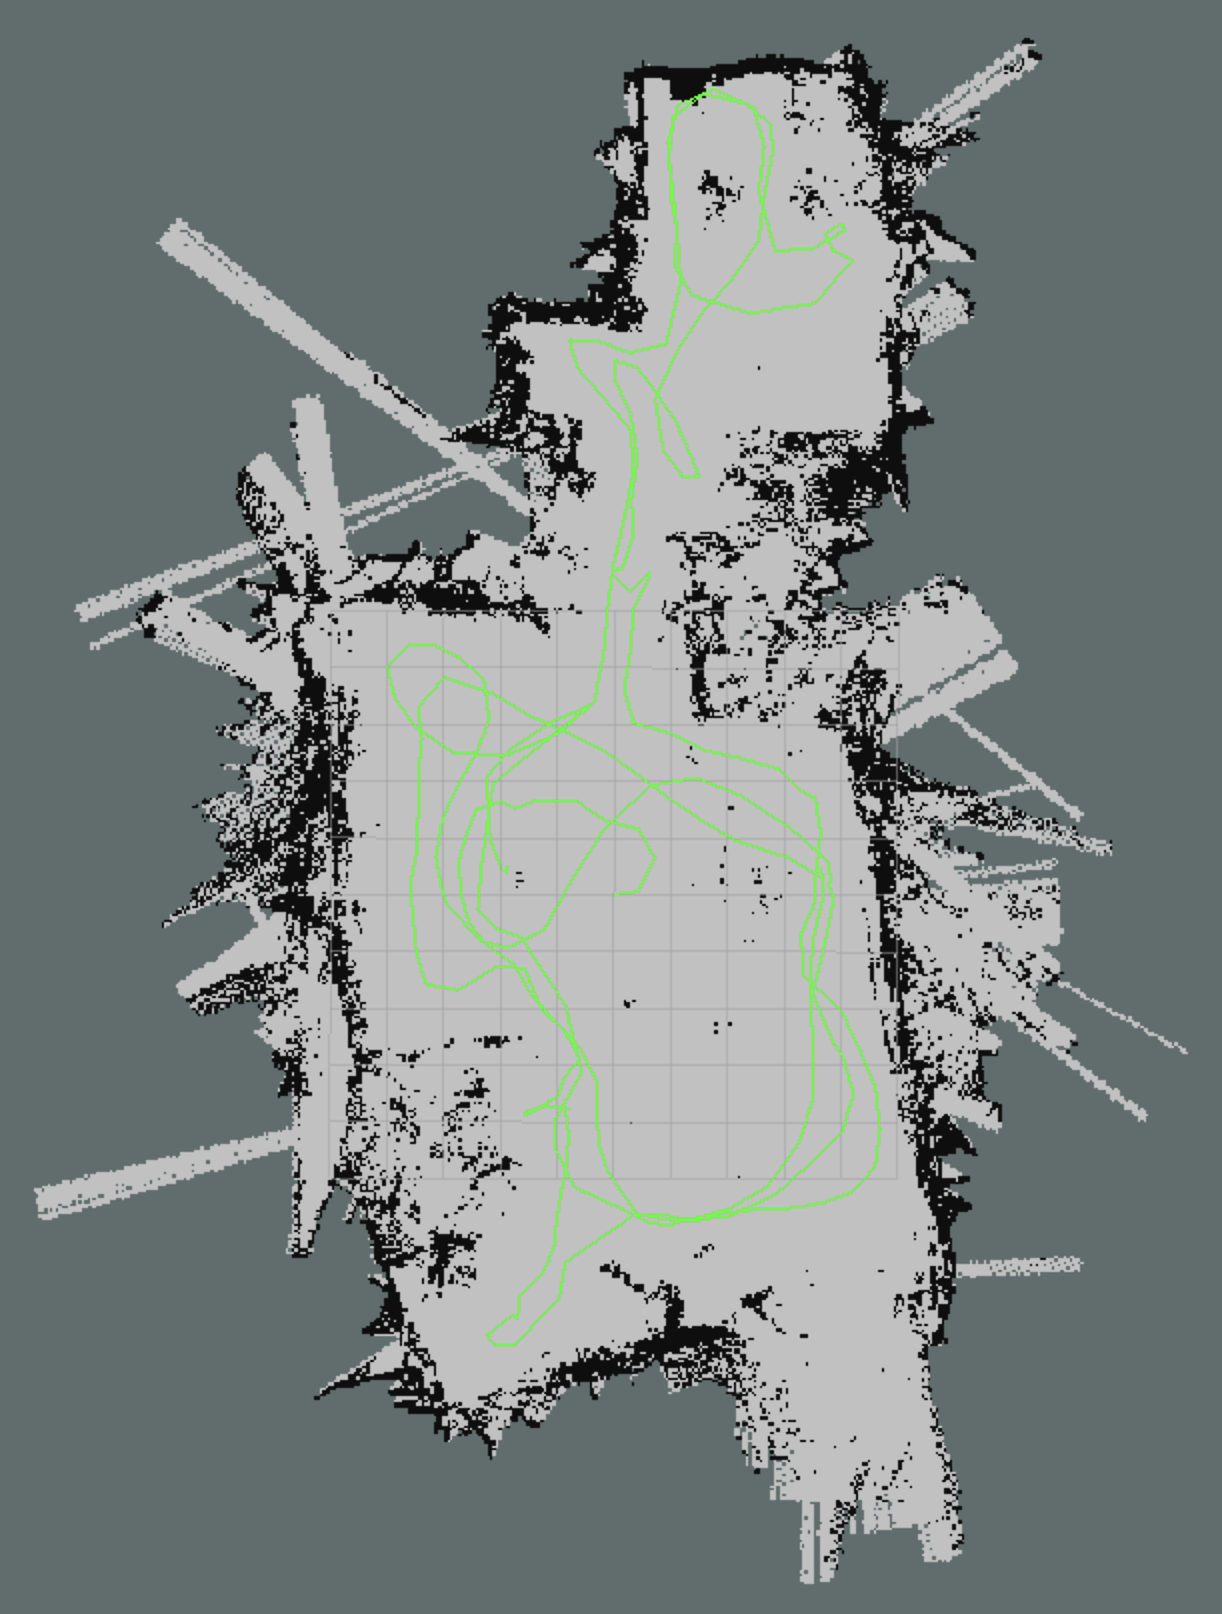
\includegraphics[width=0.8\linewidth]{img/airlabMap}
	\caption{
		Occupancy grid of the AIRLab at the HTBLuVA Wiener Neustadt including the path pursued by the drone as it got carried through the laboratory. The map as seen above is of low quality including many artefacts, sensor noise as well as misaligned proportions.
		Although the main room is poorly mapped with many error, the smaller workshop at the top is depicted relatively accurate.
	}
	\label{fig:AirLABmap}
\end{figure}

As localization and mapping data is utilized to perform real-time path-planning as well as drone control these modules are a crucial part of the Autumn Drone, thus requiring a algorithm that solves the online SLAM problem in a efficient manner while maintaining compatibility to the hardware in use. This restraints the solution in question to perform visual SLAM supporting stereo images and 6DoF-Odometry. 
While remaining within the package-space of ROS this reduces the number of potential algorithms to the following graph-based SLAM solutions:
\begin{itemize}
	\item \href{https://github.com/raulmur/ORB_SLAM2}{ORB-SLAM2}
	\item \href{https://github.com/lrse/sptam}{S-PTAM}
	\item \href{http://introlab.github.io/rtabmap/}{RTAB-Map}
	\item \href{https://felixendres.github.io/rgbdslam_v2/}{RGBDSLAMv2}
\end{itemize}

ORB-SLAM2 and S-PTAM where not selected as both approaches do not provide online occupancy grids as ROS-Topics which makes them infeasible to use and incorporate with the path-planning module of Autumn. Furthermore they do not propose a memory-management strategy thus potentially making loop-closure processing within large maps cumbersome. 

The algorithm chosen to be used for Autumn was RTAB-Map as incorporating stereo-images and external odometry is supported out-of-the-box and a variety of outputs such as 2D and 3D occupancy grids as well as a dense point cloud are offered. 
As loop-closure detection algorithm with memory management was the primary goal of RTAB-Map, it qualifies for usage in large-scale environments during long mapping sessions.
Since its publication in 2013 this algorithm has been extended and improved to support stereo- or RGBD-footage, 2D as well as 3D Lidar data and provides nodes for processing visual or lidar based odometry if no other external topic is available. 
For Autumn this approach was implemented by providing the stereo-image stream as well as visual odometry data from the Stereolabs ZED2 thus yielding in multiple occupancy grids, robot paths as visualized in Fig. \ref{fig:AirLABmap}.

Although RGBDSLAMv2 does not fully qualify to be considered in this project as it only works with RGBD-Cameras like the XBOX Kinect or Intel RealSense it is worth mentioning as it provides a 3D occupancy grid and a dense point-cloud similar to RTAB-Map.\footcite{labbe2019rtab}

%\section{Application Scenarios}
%
%\subsection{Map Acquisition}
%
%\subsection{Black-Box Localization}
%
%\subsection{Continuos Map Exploration}
%
%
%\section{2D SLAM}
%
%\subsection{Evidence Grid-based SLAM}
%
%\subsection{Graph-based SLAM}
%
%\subsection{Feature-based SLAM}
%
%
%\section{3D SLAM}
%
%\subsection{Visual SLAM}
%
%\subsection{Graph-based SLAM}
%
%
%\section{Obtaining Odometry}
%
%\subsection{Wheel Encoder Odometry}
%
%\subsection{Visual Odometry}
%
%\subsection{Visual Inertial Odometry}

\section{Topics not mentioned in this Chapter}
The SLAM problem is a highly diversified field of study with many different concepts not only concerning one paradigms adaption to other use cases than originally mentioned but also diving into the exact implementations of any of its components. Due to this abundance of concepts and algorithms it would be infeasible to characterize every one of them. 
However for the intrigued reader the author suggests the following topics and resources for further reading:
\begin{itemize}
	\item Particle Filtering for grid-based SLAM\footcite{grisetti2005ParticleGrid}
	\item Visual SLAM approaches. A wide range of literature on this topic is provided by the \href{https://vision.in.tum.de/research/vslam}{Technical University in Munich (TUM)}.
	\item Graph-SLAM frontends using different data association approaches for visual SLAM such as feature based matching like RANSAC\footcite{Jia2018FeatureMatching} or point-to-point matching like ICP\footcite{Horn1988ICP}. 
	\item Mapping in dynamic environments capable of comprehending moving obstacles within the environment\footcite{wang2003dynSLAM}
	\item SLAM with multiple robots\footcite{gutmann2003IncrMapping}
\end{itemize} 




\filbreak